\documentclass{article}
\usepackage[final]{neurips_2019}
\usepackage{morris}

% Some update to the NIPS template
\bibpunct{[}{]}{;}{n}{}{,}
\makeatletter
\renewcommand{\@noticestring}{Deep Learning, Sommer 2019, Universiteit van Amsterdam}
\makeatother

\renewcommand{\thesubsubsection}{\alph{subsubsection})}

\title{Assignment 2. Recurrent Neural Networks and Graph Neural Networks}
\author{%
  Maurice Frank\\
  11650656\\
  \href{mailto:maurice.frank@posteo.de}{maurice.frank@posteo.de} \\
  Code: \href{https://github.com/morris-frank/uvadlc_practicals_2019/tree/master/assignment_2}{github}
}

\begin{document}
\maketitle

\section{Vanilla RNN versus LSTM}
\subsection{RNN derivatives}
\begin{align}
  \pf{\L}{\B{W}_{ph}}
  &= \Π \pf{}{} \· \pf{}{\B{W}_{ph}}
\end{align}
\begin{align}
  \pf{\L}{\B{W}_{hh}}
  &= \…
\end{align}

\subsection{Vanilla RNN code}
Find the code inside \texttt{vanilla\_rnn.py} and \texttt{train.py}.

\subsection{Vanilla RNN experiment}
See Figure~\ref{fig:accuracy_loss} for a overview plot of the results and Section~\ref{sub:lstm_practice} for a discussion/comparsion of the results.

\subsection{Optimizers}
SGD has problems.
One of them is ocurring oscilattions in valleys of the loss space.
SGD does not have any \textit{memory} and thus just tries to approximate the currents face gradient to follow down which might make the path jump around a minimum of the valley.
One change to counter this problem is introducing \textbf{momentum}.
Following the intuition of the physical term, the gradient with momentum gets only changed gradually not sudden in every optimizer step.
This is implemented as a decaying average of gradient updates.
The weights get updated as a weighted sum of the previous update and the new gradient.
A second idea is to tweak the learning rate for each weight and not use a fixed \(\eta\) for all, yielding a \textbf{adaptive learning rate}.
For those weights that change a lot (bounce around some valley) we want to reduce the update step to counteract the bouncing.
This can be seen in the RMSProp~\citep{hinton2014} optimizer as described below:
\begin{align}
  v_t &= \rho v_{t-1} + (1-\rho) \· {(\nabla_{\θ_t}f)}^2\\
  \θ_{t+1} &= \θ_t - \f{\eta}{\sqrt{v_t + \ε}} \· \nabla_{\θ_t}f
\end{align}
\(\rho\) defines the decying sum. We compute the update but than divide the learning rate \(\eta\) for each weight by the new update.
Thus oscillating weights will get a smaller update.
Adam~\citep{kingma2014} optimizer works quite similar:
\begin{align}
  v_t &= \β_1 \· v_{t-1} - (1 - \β_1) \· \nabla_{\θ_t}f\\
  s_t &= \β_2 \· s_{t-1} - (1 - \β_2) \· {(\nabla_{\θ_t}f)}^2\\
  \θ_{t+1} &= \θ_t - \f{\eta}{\sqrt{s_t + \ε}} \· v_t
\end{align}
We also adapt the learning rate per weight by dividing by the square-root of the  squared gradients.
But here also directly use the momentum but having the decaying sum of weight-wise gradients. \(\β_1 \text{and} \β_2\) are tuneable hyperparameters.

\subsection{LSTM theory}
\subsubsection{LSTM Gates}
\begin{description}
  \item[\I{input modulation gate} \(\B{g}^{(t)}\)] The input modulation gate determines candidate information from the new input (using also the old hidden state).
  We want our state values normalized but need also negative values (otherwise the cell values would only increase) which, as in this case, can be done with a \(\tanh \), squashing the input to \([-1, 1]\).
  \item[\I{input gate} \(\B{i}^{(t)}\)] The input regulates which and how much information of the input of this time step should be included in the cell and hidden state.
  As the input gate regulates the flow it is necessary to have its values bounded to \([0,1]\) which can most directly achieved by squashing the values with the sigmoid.
  \item[\I{forget gate} \(\B{f}^{(t)}\)] The forget gate regulates which and how much information from the old cell state should be disregared under the new information from the input (and the old hidden state).
  As the forget gate only changes the importance (magnitude) of the information in the cell state it should be in \([0,1]\) which is achieved with the sigmoid.
  \item[\I{output gate} \(\B{o}^{(t)}\)] The output gate regulates which and how much information from the new cell state should go into the new hidden state.
  Again its gating the values from the other tensor which is asking for a range \([0, 1]\) achieved by the sigmoid.
\end{description}

\subsubsection{Number of parameters}
We have given \(\B{x}\∈\ℝ^{T\×d}\) with \(T\) sequence length and \(d\) feature dimension.
Further we have \(n\) hidden units.
Then we have
\begin{equation*}
  4\· (d\·n + n\·n + n)
\end{equation*}
trainable parameters for \textit{one} LSTM cell.
If we want to include the projection onto the classes \(c\) the size increases of course to:
\begin{equation*}
  4\· (d\·n + n\·n + n) + n\·c + c
\end{equation*}

\subsection{LSTM practice}\label{sub:lstm_practice}
Find the code inside \texttt{lstm.py} and \texttt{train.py}.
For a overview check out Figure~\ref{fig:accuracy_loss}.
We see in general that the LSTM is able to learn the palindromes faster and for longer sequences.
The RNN is only able to improve on randomness (accuracy of 0.1) up to length 17.
Further the RNN is only able to reach full accuracy for palindromes smaller than 10.
The LSTM learns for all lengths but we see that for length of 23 we do not see improvement over randomness until almost 3000
(if run for lon enough the LSTM learns full accuracy for all tested lengths but we found that not be the interesting result here).
This is explained in that we use the same hyperparameters for all experiments expecially the learning rate.
An optimization of the hyperparameters for the LSTM might speed up training for longer sequences.
The experiment clearly shows that the LSTM is more capable of learning longer dependencies.

\begin{figure}
  \centering
  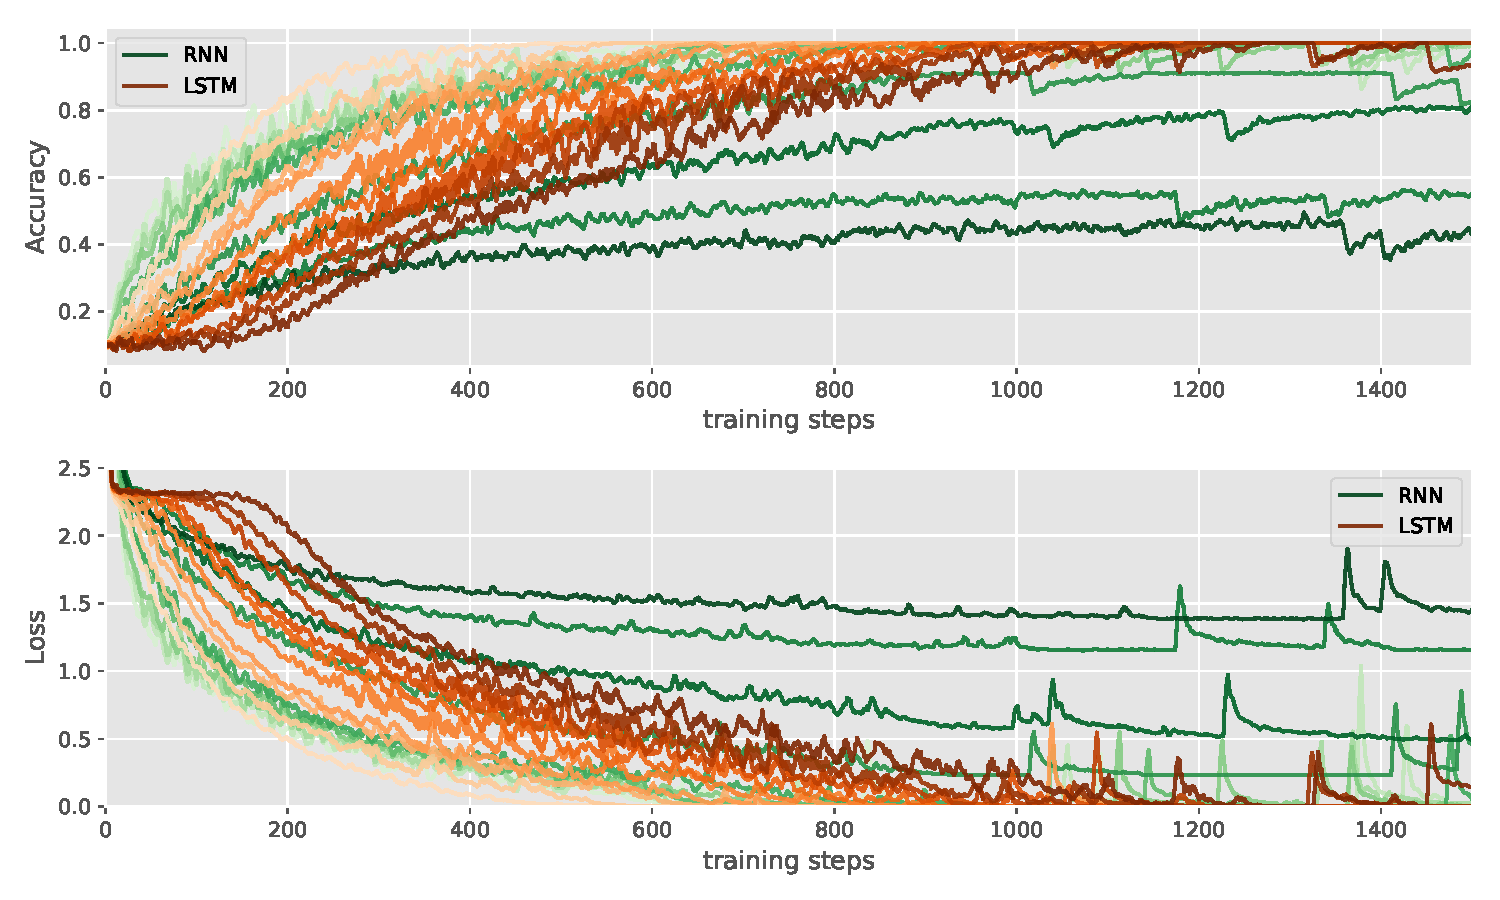
\includegraphics[width=\linewidth]{assignment_2/part1/palindrome.pdf}
  \caption{\B{Top} the accuracy and \B{bottom} the loss while training.
  Color lightness codes the palindrome length ranging from 5 numbers with the lightest color in steps of 2 to 23 numbers with the darkest color.
  (Making 9 curves per model). All curves are an average of ten runs and smoothed with a box filter of size 10 for better radibility.}\label{fig:accuracy_loss}
\end{figure}

\section{Recurrent Nets as Gernerative Model}
\subsection{Learning South Park}
\subsubsection{The code}
Find the code inside \texttt{model.py} and \texttt{train.py}.

\subsubsection{}
\subsubsection{}
\subsection{}

\section{Graph Neural Networks}
\subsection{Forward Layer}
\subsubsection{}
The \(\hat{A}\) matrix contains the edge information between the nodes in the graph.
This includes the self-connections of all nodes from the identity \(\1_N\).
We update the activations with \(H^{l+1} = \σ(\hat{A}H^{(l)}W^{(l)})\).
So we update the activation associated with one node only for the activations of edges that have non-zero edge weights in \(\hat{A}\).
A node is changed by the nodes its connected to.
In reverse we can see that information in one node can propagate to all connected adjacent nodes in one time step which can be visualized as the message passing over the graph.

\subsubsection{}
In every layer of the GCN you can propagate information along one edge so to let information reach a node three hops away we would need three layers.

\subsection{Applications of GNN}
In \textit{Multi-Granularity Reasoning for Social Relation Recognition from Images}~\cite{zhang2019} the authors build graphs on images of humans.
The graphs describe first the relationship of a person in the image with its surrounding objects amongst other things other persons in the image.
A second graph represents the pose of each person in the image.
On these two types of graphs they use Graph Convolutional Networks (GCN) to predict the social relationship of these persons.
For example in an image of parent and child the bending pose of the parent and the connection of the two persons in the Person-Object graph lets the method infer their relationship.

Next in \textit{Disease Prediction using Graph Convolutional Networks: Application to Autism Spectrum Disorder and Alzheimer's Disease}~\cite{parisot2018} propose to use GCN for medical image processing.
The nodes of the graph in this setting are features of medical image acquisitions which in their experiments are gathered from structural and functional MRI.
As they predict the health state of multiple individuals at once the graph consists of many image features of multiple persons.
The edges here describe the phenotypical similarity between two individuals which are described by categorical medical data (e.g.\ sex).
The GCN uses this graph to predict the health state of the population.


Lastly in \textit{Temporal Relational Ranking for Stock Prediction}~\cite{feng2019} we seen an application of GCN in stock prediction.
Here the nodes are features capturing the historical information of one stock and the edges capture the relations between two companies stock.
Both historical intra and inter stock features are generated by LSTM from historical stock data.
Again we build a graph from the edges and nodes and use GCN to predict in this case the stocks next day performance at the market.

\subsection{Comparsion adn Combination of GNN and RNN}
\subsubsection{}
Generally a graph structure is necessary for non-Euclidean spaces.
\subsubsection{}

\bibliographystyle{unsrtnat}
\bibliography{references}

\end{document}
